% \begin{itemize}
%     \item Network connectivity, E/I balance, raster plots
%     \item Too many possible connections to test them all → Subsampling
%     \item Performance of last chapter's methods
%     \item If time: experiment with a network that is less densely connected than our current fully-random one. Why? To better examine the effect of indirect connections / colliders (For the current connectivity, there are too many of those. But in a more realistic, 'localized' network, there are less, and so it seems easier to isolate and examine their effect).
% \end{itemize}

\section{Introduction}

In the previous experiments, only one neuron's voltage was simulated. The inputs were Poisson spike trains.
In the next experiments, we simulate the voltages of a full network of neurons, which are recurrently connected to each other.
The goal is to investigate the effect on network inference of potentially correlated inputs and indirect connections.




\section{Connectivity structure}

\begin{figure}
    \subfloat{
        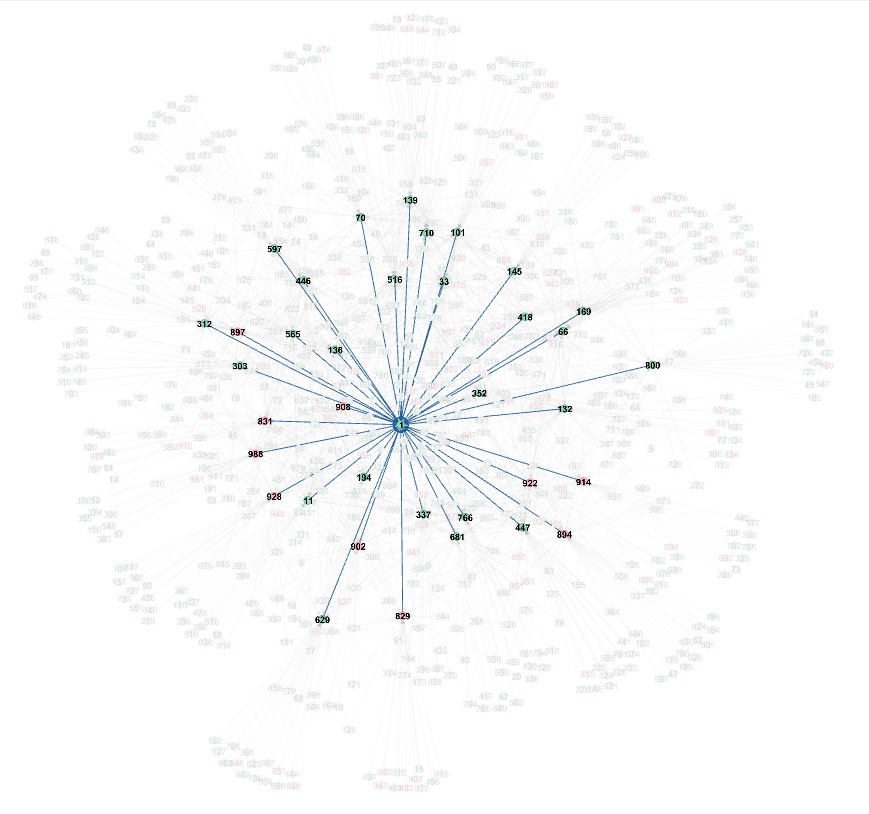
\includegraphics[w=0.75]{gephi-direct-inputs.png}
        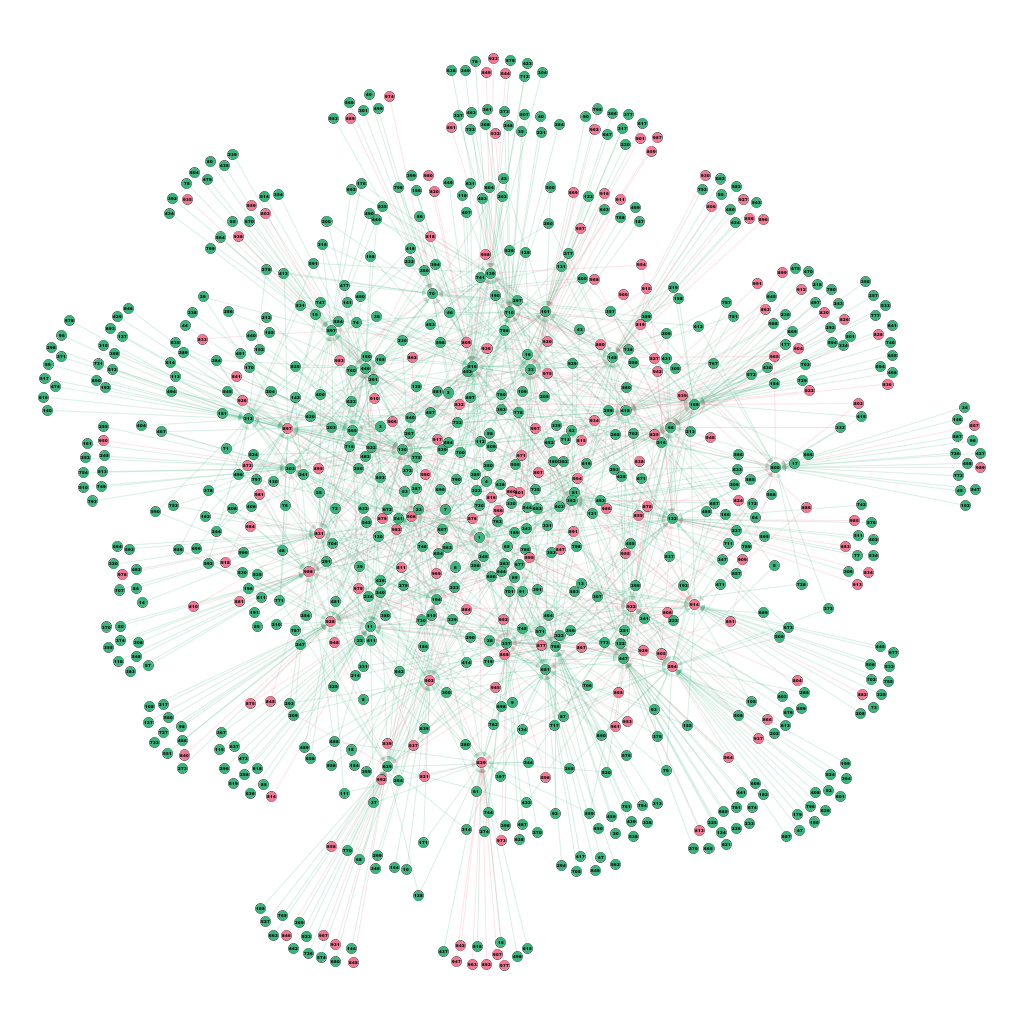
\includegraphics[w=0.75]{gephi-inputs-to-inputs.png}
    }
    \vspace*{2em}
    \caption
        {\textbf{A neuron is reachable in two hops from most other neurons}.    Selected neurons and connections in our random network. Left shows the direct inputs to one of the neurons. Right additionally shows the direct inputs to these inputs. This subnetwork already contains more than 700 of the 1000 total neurons in the network.\\
        Excitatory neurons in green, inhibitory in red. The tangle in the middle consists of neurons that synapse onto multiple of the direct inputs of our selected neuron.\\
        Visualization using the `Gephi' software, with the `Yifan-Hu' layout algorithm, and default parameters otherwise.
        Source: \nburl{2022-08-29__Visualizing_subnets}.}
    \label{fig:gephi-network-viz}
\end{figure}

% These two margin figs can go to Appendix
\marginpar{
    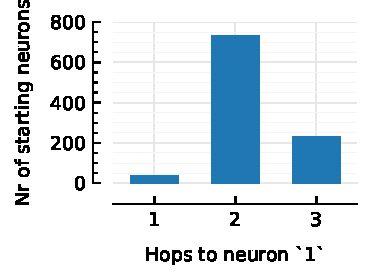
\includegraphics[w=1, trim={0 0.4em 0 -1em}, clip]{shortest-path-1}
    \captionof{figure}{
        \textbf{A selected neuron is reachable in at most three hops.}
        Shortest path lengths from every other neuron in the network.}
    \label{fig:shortest-path-1}
}
\marginpar{
    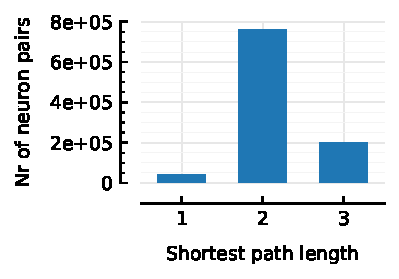
\includegraphics[w=1, trim={0 0.4em 0 -1em}, clip]{shortest-path-all}
    \captionof{figure}{
        \textbf{Every neuron is reachable in at most three hops.}
        Shortest path lengths calculated using the Floyd-Warshall algorithm. Source: \nburl{2022-07-14__Unconnected-but-detected.html}.}
    \label{fig:shortest-path-all}
}

We choose the simple and common `fully random' connectivity rule,\footnote{
    Other common choices for connectivity structure are scale-free networks, and `local' networks.
}
where any neuron has a connection to another with a uniform random probability (we choose $p_\text{conn} = 0.04$). After generating an adjacency matrix this way (\verb|A = rand(N, N) .≤ 0.04|, where \verb|rand| draws from $\sim U[0,1]$), we remove autapses. We choose the number of neurons $N = 1000$.

A property of fully random networks is that they are strongly interconnected. In our network, any neuron is reachable from any other in at most three steps (three synapses); most are reachable in just two. This is exemplified in \cref{fig:gephi-network-viz} and \cref{fig:shortest-path-1}: one selected neuron (neuron `1' here) is reachable in two hops from more than 700 of the 1000 total neurons in the network. And when we compute the shortest path between every possible neuron pair, we find a very similar distribution (\cref{fig:shortest-path-all}).




\section{External input}

As we no longer have Poisson spike trains providing input to our neurons, we need another way of bootstrapping activity in the network.\\
Instead of external spikes, each neuron is provided with external input by adding Gaussian noise to its membrane voltage. Every time step ($Δt = 0.1$~ms), a sample drawn from a normal distribution with mean $–0.5$~pA and $σ = 5$~pA is added to the membrane current. (As membrane current is by convention negative, this corresponds to an on-average positive influence on membrane voltage).



\section{EI balance}

Similar to the N-to-1 experiments, we make 1 out of 5 neurons inhibitory.
As before, this is done by setting the synaptic reversal potential at the outputs of inhibitory neurons to $-80$ mV (instead of the $0$ mV for excitatory neurons).
To make sure that each neuron receives a balanced mix of excitation and inhibition, and given that there are 4:1 excitatory to inhibitory neurons, we make excitatory neurons 4x weaker: their synaptic strength ($Δg$, the instantaneous increase in postsynaptic conductance $g$ on spike arrival) is 4x as small as that of inhibitory neurons.



\section{Subsampling}

We simulate all 1000 neurons' voltages, but, to save memory and disk space,  do not record all these traces.\footnote{
    For a 10-minute simulation with a timestep of 0.1 ms, one voltage trace takes 48 MB (at 64 bit per sample). Our 1000 neurons thus take 48 GB -- and that is just for one simulation (one set of parameters).\newline
    We \emph{do} record the spike trains of all neurons. Saving just spike times takes considerably less space: a neuron spiking at 10 Hz for 10 minutes emits 6000 spikes, which, at 64 bit per timestamp, takes just  48 kB.\newline
    In other words,  at a 0.1 ms sample rate, a spike train occupies about 1000× less memory than the corresponding voltage trace.
}
In most experiments here, we recorded the voltage traces of 40 excitatory and 10 inhibitory neurons (5\% of all neurons).

Additionally, when performing connection tests on the inputs of a recorded neuron, we do not test the spiketrains of all 999 other neurons. Instead, we test only a (biased) sample of the possible inputs, to save processing time.
This sample is constructed as follows. We test all the a-priori known true direct inputs -- both excitatory and inhibitory -- and add a random sample of 40 not-directly-connected neurons.

On average, each neuron has ± 32 excitatory inputs and ± 8 inhibitory inputs. This means that, from the 1000 × 1000 possible connections, we only test about 4000, or 0.4\%.\footnote{
    Calculation behind these numbers:\\
    - 1000 neurons × 80\% excitatory × 4\% probability of an input connection = 32 excitatory inputs on average.\\
    - 50 `post' neurons (40 excitatory and 10 inhibitory voltage-recorded neurons) × 80 `pre' neurons (±40 connected + 40 unconnected) = 4000 tested connections.\\
    - To be precise, instead of 1000 × 1000, there are rather  $1000^2 - 1000$ possible connections, as we would not test for autapses.
}

\begin{figure}
    \subfloat{
        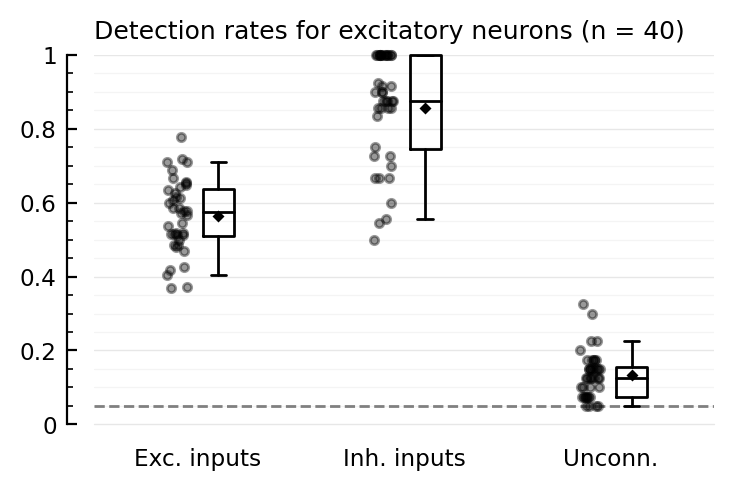
\includegraphics[w=0.74]{2022-09-01__1144_weights_23_0.png}
        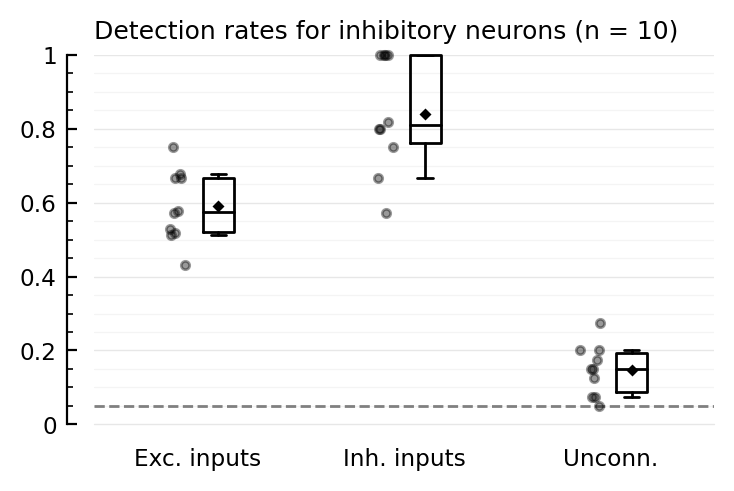
\includegraphics[w=0.74]{2022-09-01__1144_weights_24_0.png}
    }
    \captionn[. ]
    {Performance of the STA `peak-to-peak' connection test in the random network}
    {10 minute recording. Each dot is the true positive rate for one`post' neuron. The gray dotted line indicates the p-value threshold α of 0.05.}
    \label{fig:net-perf}
    \vspace*{2em}
\end{figure}
